\section{CAPÍTULO I: Diagnóstico de la solución}

\subsection{Planteamiento del problema}

El sistema educativo actual enfrenta un desalineamiento crítico entre las tareas académicas asignadas por los profesores y la percepción de relevancia que tienen los estudiantes sobre estas actividades. Hoy en día, muchos estudiantes se enfrentan a un problema fundamental: los profesores asignan tareas de investigación y actividades académicas, pero los alumnos sienten que estas no les servirán en su vida real \cite{deci2017}. Esta desconexión entre el aprendizaje académico y la aplicabilidad percibida genera que los estudiantes prioricen aprobar antes que aprender genuinamente.

Como consecuencia de esta problemática, los estudiantes recurren sistemáticamente al uso inadecuado de herramientas digitales disponibles para resolver tareas sin realmente adquirir conocimiento sobre el tema. Utilizan buscadores para copiar información sin procesarla, herramientas de inteligencia artificial para generar respuestas completas sin análisis crítico, y plataformas digitales para transcribir contenido sin comprenderlo \cite{martinez2023}. Este comportamiento transforma las herramientas tecnológicas, que deberían ser facilitadores del aprendizaje, en atajos para cumplir con requisitos académicos sin lograr una comprensión real del contenido \cite{chen2023}.

\subsubsection{Situación actual del comportamiento académico estudiantil}

El análisis del comportamiento estudiantil actual revela patrones preocupantes en la forma como los estudiantes abordan las tareas académicas y utilizan las herramientas digitales disponibles:

\paragraph{Priorización de la aprobación sobre el aprendizaje}
Los estudiantes han desarrollado una mentalidad enfocada únicamente en obtener calificaciones aprobatorias, independientemente de si han adquirido conocimiento real sobre el tema. Esta orientación hacia el resultado inmediato genera que busquen el camino más eficiente para cumplir con los requisitos académicos, sin importar si comprenden o no el contenido \cite{sappaile2024}.

\paragraph{Uso inadecuado de herramientas digitales como atajos}
Las herramientas tecnológicas disponibles se han convertido en medios para evitar el proceso de aprendizaje genuino. Los estudiantes utilizan motores de búsqueda para copiar información textualmente, emplean herramientas de inteligencia artificial para generar ensayos completos sin leerlos, y recurren a plataformas digitales para obtener respuestas inmediatas sin desarrollar habilidades de pensamiento crítico \cite{martinez2023}.

\paragraph{Desconexión entre tareas académicas y relevancia práctica}
Existe una percepción generalizada entre los estudiantes de que las tareas asignadas carecen de aplicabilidad en su vida cotidiana o futura carrera profesional. Esta desconexión fomenta el desinterés y justifica, desde su perspectiva, el uso de atajos para completar las actividades sin involucrarse genuinamente con el contenido \cite{nurhayati2025}.

\paragraph{Aprendizaje superficial sin comprensión profunda}
El patrón de comportamiento actual resulta en un aprendizaje superficial donde los estudiantes memorizan información temporalmente para superar evaluaciones, pero no desarrollan una comprensión profunda ni retienen conocimientos a largo plazo. Este enfoque superficial limita el desarrollo de habilidades de análisis, síntesis y aplicación del conocimiento \cite{rahmi2025}.

\paragraph{Falta de motivación intrínseca hacia el conocimiento}
La ausencia de elementos motivadores intrínsecos en las metodologías educativas tradicionales genera que los estudiantes no encuentren satisfacción personal en el proceso de aprender. Sin esta motivación intrínseca, recurren naturalmente a herramientas que les permitan cumplir con las obligaciones académicas con el mínimo esfuerzo cognitivo posible \cite{coelho2025}.

\begin{figure}[H]
	\centering
	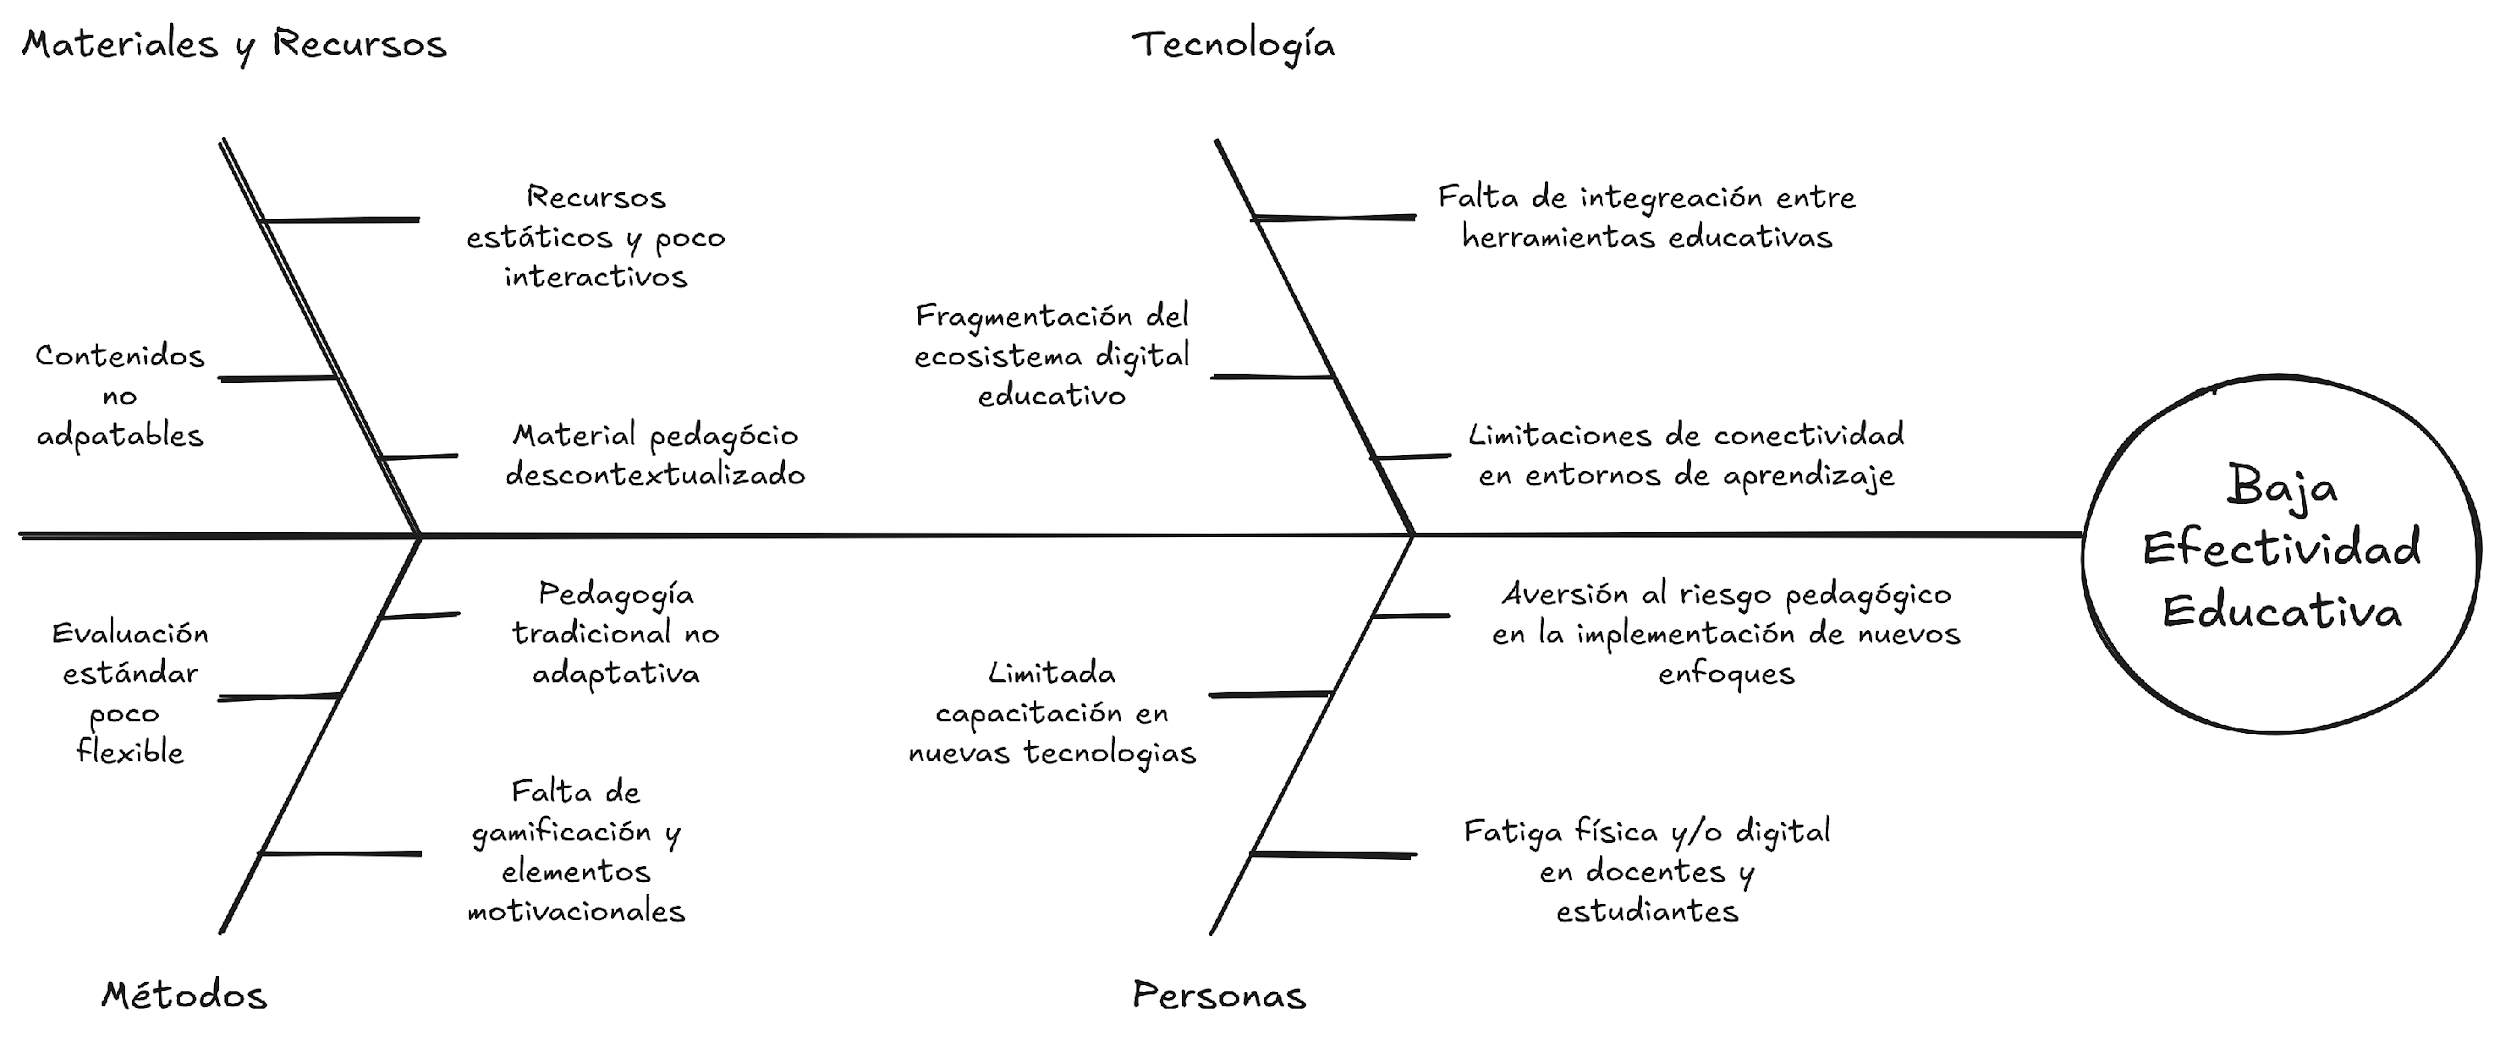
\includegraphics[width=0.9\textwidth]{images/diagrama_de_ishikawa.png}
	\caption{Diagrama Ishikawa: Causas de ineficiencia en el sistema tradicional.}
	\label{fig:ishikawa}
\end{figure}

El diagrama de Ishikawa muestra de manera sistemática las múltiples causas que contribuyen a la ineficiencia del sistema educativo tradicional, categorizando los factores en aspectos metodológicos, tecnológicos, motivacionales y estructurales.

\subsubsection{Análisis de las Causas del Problema Educativo Actual}

\paragraph{CAUSA 1: Disponibilidad irrestricta de herramientas para atajos académicos}
El acceso inmediato y sin restricciones a motores de búsqueda, herramientas de inteligencia artificial generativa, y plataformas de resolución de tareas ha creado un entorno donde los estudiantes pueden obtener respuestas completas sin necesidad de procesar información o desarrollar habilidades de pensamiento crítico. Esta disponibilidad tecnológica, aunque potencialmente beneficiosa para el aprendizaje, se ha convertido en una barrera cuando se utiliza como sustituto del proceso de aprendizaje genuino \cite{saputra2025}.

\paragraph{CAUSA 2: Ausencia de metodologías que transformen herramientas digitales en facilitadores de aprendizaje}
Las metodologías educativas actuales no han evolucionado para integrar efectivamente las herramientas digitales disponibles como parte del proceso de aprendizaje. En lugar de diseñar experiencias que aprovechen estas tecnologías para profundizar la comprensión, las instituciones educativas mantienen enfoques tradicionales que no consideran el potencial educativo de las herramientas digitales, creando una desconexión entre la realidad tecnológica de los estudiantes y las expectativas académicas \cite{nurhayati2025}.

\paragraph{CAUSA 3: Falta de elementos motivadores intrínsecos en las tareas académicas}
Las actividades académicas tradicionales carecen de elementos que generen motivación intrínseca en los estudiantes. Sin componentes como desafíos progresivos, retroalimentación inmediata, reconocimiento de logros, o conexión clara con aplicaciones prácticas, los estudiantes no encuentran razones convincentes para involucrarse genuinamente con el contenido académico, lo que los lleva a buscar alternativas que les permitan cumplir con menor esfuerzo \cite{sappaile2024}.

\subsection{Objetivos del proyecto}

\subsubsection{Objetivo general}

Desarrollar una aplicación educativa 3D gamificada que transforme las herramientas digitales de atajos académicos en facilitadores genuinos del aprendizaje, incrementando la motivación intrínseca y el compromiso estudiantil con el contenido académico a través de experiencias de aprendizaje inmersivas y relevantes.

\subsubsection{Objetivos específicos}

\begin{itemize}
\item Diseñar y desarrollar un entorno virtual 3D inmersivo que convierta las tareas académicas tradicionales en experiencias de aprendizaje motivadoras y significativas, donde los estudiantes perciban la relevancia práctica del conocimiento adquirido.
\item Implementar mecanismos de gamificación que fomenten el uso productivo de herramientas digitales, transformándolas de atajos para aprobar en instrumentos que profundicen la comprensión y desarrollen habilidades de pensamiento crítico.
\item Crear un sistema de progresión y recompensas que genere motivación intrínseca hacia el aprendizaje, donde el proceso de adquirir conocimiento sea tan atractivo como obtener la calificación final.
\item Desarrollar integraciones con plataformas educativas existentes que permitan a los docentes crear experiencias de aprendizaje que aprovechen las herramientas digitales disponibles como parte integral del proceso educativo, no como sustitutos del mismo.
\end{itemize}

\subsection{Alcance de la solución}

La plataforma educativa interactiva 3D para la gamificación de tareas académicas abarca:

\paragraph{Componentes funcionales}

\begin{itemize}
\item Sistema de registro y autenticación segura para administradores, docentes y estudiantes, con diferentes niveles de acceso según rol y responsabilidades.
\item Entorno virtual 3D inmersivo que simula un mundo medieval, con personajes interactivos, escenarios dinámicos y elementos visuales atractivos que contextualizan las actividades educativas.
\item Módulo de creación y gestión de tareas gamificadas que permite a los docentes configurar actividades educativas como misiones, retos y aventuras dentro del entorno virtual.
\item Sistema de evaluación y retroalimentación inmediata que convierte la evaluación tradicional en un proceso dinámico y motivador integrado a la narrativa del entorno.
\item Sistema de recompensas y progresión que incentiva la participación constante y reconoce los logros académicos.
\item Sistema de notificaciones vía push, correo electrónico, Discord y dentro de la plataforma para mantener informados a todos los usuarios sobre nuevas tareas, plazos y eventos.
\end{itemize}
